\chapter{Background}\label{ch:Background}
This chapter presents some background information. Some theorem and formulas that I will be used in the algorithm later is also mentioned here. The situation of image registration is first introduced as the application scenario of the algorithm. And the algorithm bases on the multiple homography, it is also a section of this chapter. Finally, the main mathematical theorem related to my algorithm is shown in the end.

\section{Image Registration}
Image registration is the process of transforming different sets of data for the same scene, which may be multiple images taken at different times, from different viewpoints, and/or by different sensors,  into one coordinate system. Almost all large systems that evaluate images require image registration, or closely related operations on the images, as an intermediate step, in which the final information is gained from the combination of various data sources like in image fusion, change detection, and multichannel image restoration.

Specific applications include, but are not limited to remote sensing (example \cref{fig:image registration example}) (Land monitoring, multi-spectral classification, change detection,  weather forecast, map updating, create super-resolution image, compiling and analyzing images and data from satellites), computer vision (image mosaicing, motion detection, automatic target localization )  and medical imaging (example \cref{fig:image registration example 2}) (monitoring tumor growth, treatment verification, comparison of the patient’s data with anatomical atlases).
\begin{figure}[htbp]
	\centering
	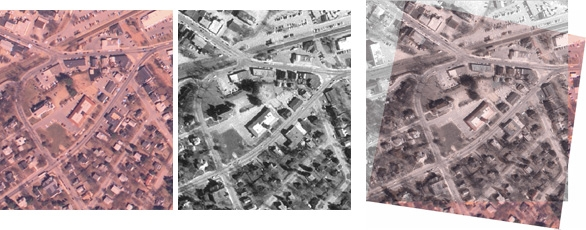
\includegraphics[width=0.80\textwidth]{images/Registering_aerial_photos}
	\caption{Registering aerial photos (\copyright\ MathWorks)}
	\label{fig:image registration example}
\end{figure}
\begin{figure}[htbp]
	\centering
	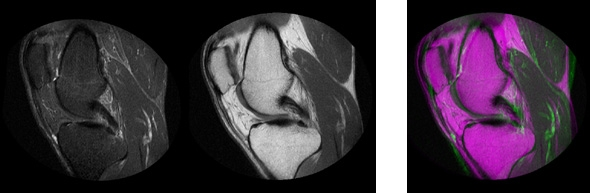
\includegraphics[width=0.80\textwidth]{images/medical_image}
	\caption{Automatic registration on multimodal medical images (\copyright\ MathWorks)}
	\label{fig:image registration example 2}
\end{figure}
In the past few decades, image acquisition devices have developed rapidly, so that the number and diversity of images obtained have increased correspondingly, which has led to the study of image registration. A comprehensive survey of image registration methods has been published in 2003 by Barbara \cite{zitovaImageRegistrationMethods2003}. Typically, the process of the most image registration technology is as follows: 
\begin{itemize}
	\item \textit{Feature detection}: Salient and distinctive objects (closed-boundary regions, edges, contours, line intersections,
corners, etc.) are manually or, preferably, automatically detected. For further processing, these features can be represented by their point representatives (centers of gravity, line endings, distinctive points).
	\item \textit{Feature matching}: The connection between corresponding features in image pair is established through this step with various feature descriptors or similarity measures along with spatial relationships.
	\item \textit{Transform model estimation}: The coordinate transformation so-called mapping function is estimated by matching features.  Image registration is performed by the mapping function.
	\item \textit{Image resampling and transformation}: In this step, one image is transformed by mapping function to another. Image values in non-integer coordinates are computed by the appropriate interpolation technique.
\end{itemize} 

\begin{figure}[htbp]
	\begin{center}
	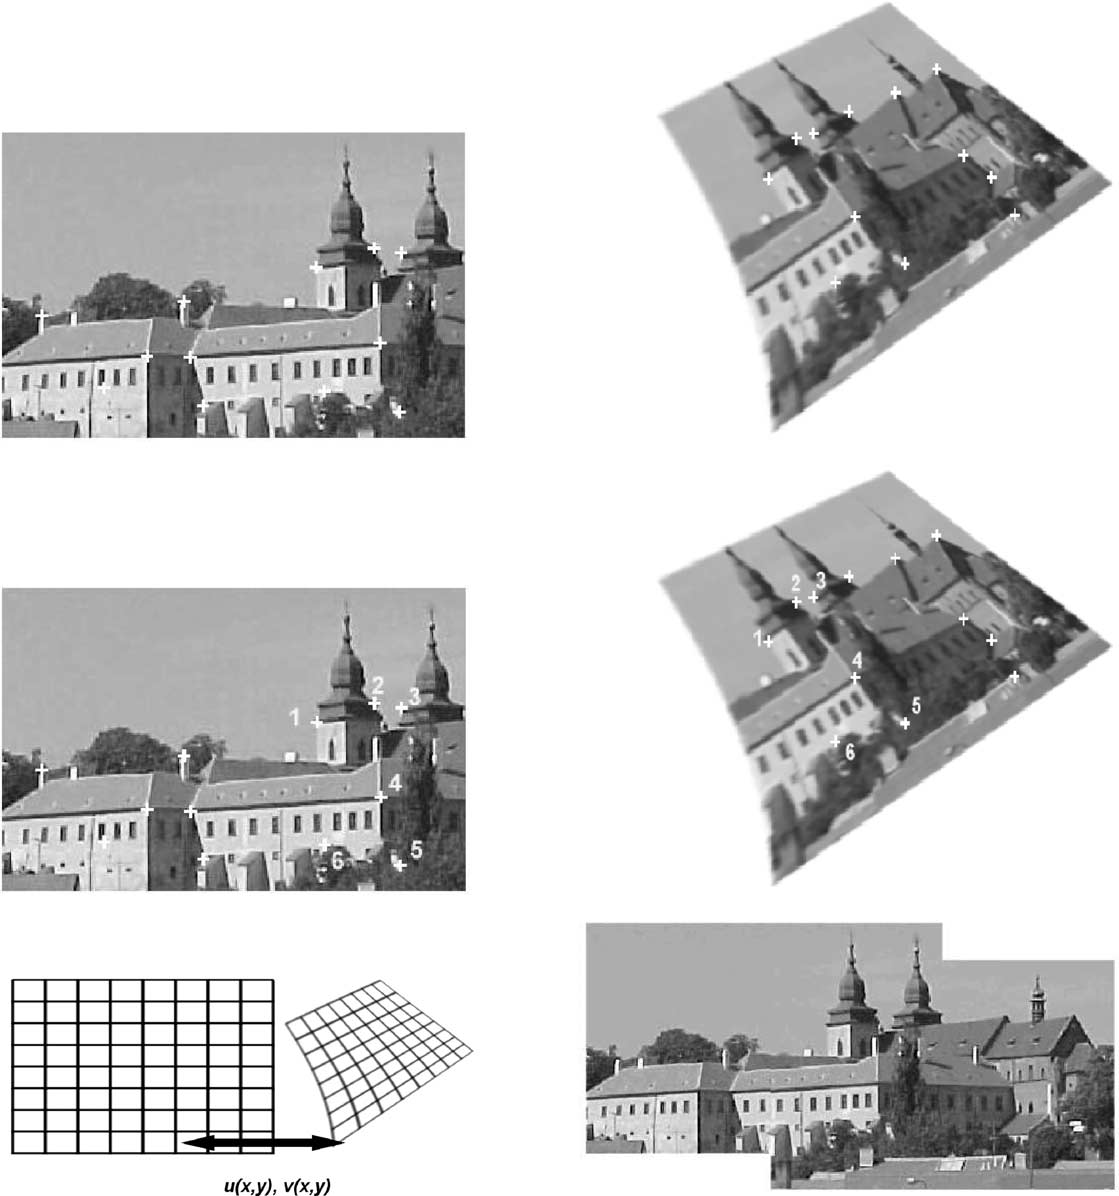
\includegraphics[width=0.80\textwidth]{images/image registration}
	\caption{Four steps of image registration}
	\label{fig:image registraion}
	\end{center}
	{\small  Top row -- feature detection (corners were used as the features in this case). Middle row -- feature matching by invariant descriptors (the corresponding pairs are marked by numbers). Bottom left -- transform model estimation exploiting the established correspondence. Bottom right -- image resampling and transformation using appropriate interpolation technique. \cite{zitovaImageRegistrationMethods2003}}
\end{figure}

Based on years of development, the current main theories of image registration can be divided into two categories: some typical dense methods seen in \cref{tab:Dense Method} and some typical sparse methods seen in \cref{tab:Sparse Method}.

\begin{table}[htbp]
	\centering
	\scriptsize  
	\begin{tabular}{p{50pt} p{300pt}}
		\toprule
		\multicolumn{2}{c}{\bfseries Dense Method}\\ \midrule
		  SGM   &  Semi-Global Matching method  performs pixel-wise matching based on Mutual Information and the approximation of a global smoothness constraint. \cite{hirschmullerAccurateEfficientStereo2005}     \\
		Correlation based Method  &  Cross-correlation is the basic statistical approach to registration. It is often used for template matching or pattern recognition in which the location and orientation of a template or pattern are found in a picture. \cite{gruenAdaptiveLeastSquares1985a}       \\ \bottomrule
	\end{tabular}
	\caption{Dense Method}  
	\label{tab:Dense Method} 
\end{table}

\begin{table}[htbp]
	\centering
	\scriptsize  
	\begin{tabular}{p{50pt} p{300pt}}
		\toprule
		\multicolumn{2}{c}{\bfseries Sparse Method}\\ \midrule
		SIFT   &  The scale-invariant feature transform (SIFT) is a feature detection algorithm in computer vision to detect and describe local features in images \cite{loweObjectRecognitionLocal1999}   \\
		ORB  &  Oriented FAST and rotated BRIEF (ORB) is a fast robust local feature detector, that  is based on the FAST key-point detector and a modified version of the visual descriptor BRIEF (Binary Robust Independent Elementary Features). \cite{rubleeORBEfficientAlternative2011}      \\ \bottomrule
	\end{tabular}
	\caption{Sparse Method}  
	\label{tab:Sparse Method} 
\end{table}

But sometimes, it's hard to tell them apart. For example, image stitching with SIFT features used the sparse feature points to estimate a dense homography. P. Hellier use simultaneously both dense and landmark-based approaches for nonrigid registration. \cite{hellierCouplingDenseLandmarkbased2003}. The Algorithm in the thesis first estimate the multiple homography matrix based on different plane patches in the image, then this series of transformation matrices could be seen as a  multiple homography matrices that is used to register the whole image..

\section{Homography} \label{sec: Multiple Homography}
The homography is a projective linear mapping, a special case of the mapping between the images of corresponding points, when those are the image points of 3D planar scene. A 2D point $\left( x, y \right)$ in an image can be represented as a 3D vector $ \rdx = \left( x_{1}, x_{2}, x_{3}\right)$ where $ x = \frac{x_{1}}{x_{3}} $ and $ y = \frac{x_{2}}{x_{3}} $. This is called the homogeneous representation of a point and it lies on the projective plane $ \dsP^{2} $ \cite{szeliskiComputerVisionAlgorithms}.  As mentioned above,  a homography is an invertible mapping of points and lines on the projective plane $ \dsP^{2} $.Other terms for this transformation include \textit{collineation}, \textit{projectivity}, and \textit{planar projective transformation}. Hartley and Zisserman \cite{hartleyMultipleViewGeometry2004} provide the specific definition that a homography is an invertible mapping from $ \dsP^{2} $ to itself such that three points lie on the same line if and only if their mapped points are also collinear. They also give an algebraic definition by proving the following \cref{thm:homography}. This tells us that in order to calculate the homography that maps each $ \rdx_{i} $ to its corresponding $ \rdx_{i}^{'} $ it is sufficient to apply a  $ 3 \times 3 $  matrix $ H $ to $\rdx_{i}$. For more mathematical derivation process, see \cref{sec:main idea}
\begin{theorem}[Homography]\label{thm:homography}
	A mapping from $\dsP^{2}\rightarrow\dsP^{2}$ is a projectivity if and only if there exists a non-singular $3\times3$ matrix $H$ such that for any point in $\dsP^{2}$ represented by vector $\rdx$ it is true that its mapped point equals $H\rdx$.
\end{theorem}

Homography have many applications in computer vision and photogrammetry: image registration, image rectification, mosaicing (\cref{fig:Homography application}) and estimation of camera motion. After extracting the camera motion from the estimated homography matrix, this information can be used for navigation, camera calibration, or to insert a 3D object model into an image or video.  The result of the proposed algorithm with the multiple homography could also be used to fundamental matrix estimation and following camera path.
\begin{figure}[htbp]
	\centering
	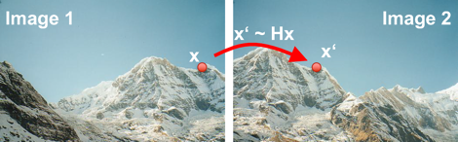
\includegraphics[width=0.80\textwidth]{images/homography_application}
	\caption{Homography application: Panorama \cite{stricker2DProjectiveTransformations2020}}
	\label{fig:Homography application}
\end{figure}

But in some situations, like remote sensing,  there are more than one flat planes in images (here mostly refers to the surface of earth) or the planes in images are not flat enough to be one plane. According to the definition of homography it can only be used for one flat plane and more than one homography matrix are needed for this case.  And this whole array of homography matrices are all intrinsically interconnected by latent variables, called multiple homography (More mathematical derivation can be found in \cref{subsec: Multiple Homography calculation}) . The algorithm is to find a set of compatible homographies between images pair.

\section{Epipolar Geometry}\label{sec:Epipolar Geometry}
The Epipolar geometry between two views is essentially the geometry of the intersection of the image planes with the pencil of planes having the baseline as axis (the baseline is the line joining the camera centres). This geometry is usually motivated by considering the search for corresponding points in stereo matching.

\cref{fig:epipolar} shows how a pixel in one image $ \rdx_{0}$ projects to an \textit{epipolar line segment} in the other image. The segment is bounded at one end by the projection of the original viewing ray at infinity $ \rdp_{\infty}$ and at the other end by the projection of the original camera center $ \rdc_{0}$ into the second camera, which is known as \textit{epipole} $\rde_{1}$. If we project the epipolar line in the second image back into the first, we get another line (segment), this time bounded by the other corresponding \textit{epipole} $\rde_{0}$. Extending both line segments to infinity, we get a pair of corresponding \textit{epipolar lines} \cref{fig:epipolar}, witch are the intersection of the two image planes with the \textit{epipolar plane} that passes through both camera centers $ \rdc_{0}$ and $ \rdc_{1}$ as well as the point of interest $ \rdp$.

Supposing now that we know only $ \rdx_{0}$, we ask how the corresponding point $ \rdx_{1}$  is constrained. The \textit{Epipolar plane} is determined by the baseline and the object $ \rdp$. From above we know that the point $ \rdx_{1}$ must lie on the line of intersection $\vec{l}_{1}$ of the \textit{epipolar plane} with the second image plane, exactly the \textit{epipolar lines} mentioned above. 
\begin{figure}[htbp]\centering
	\subfloat[]{
		\label{fig:epipolar_1}
		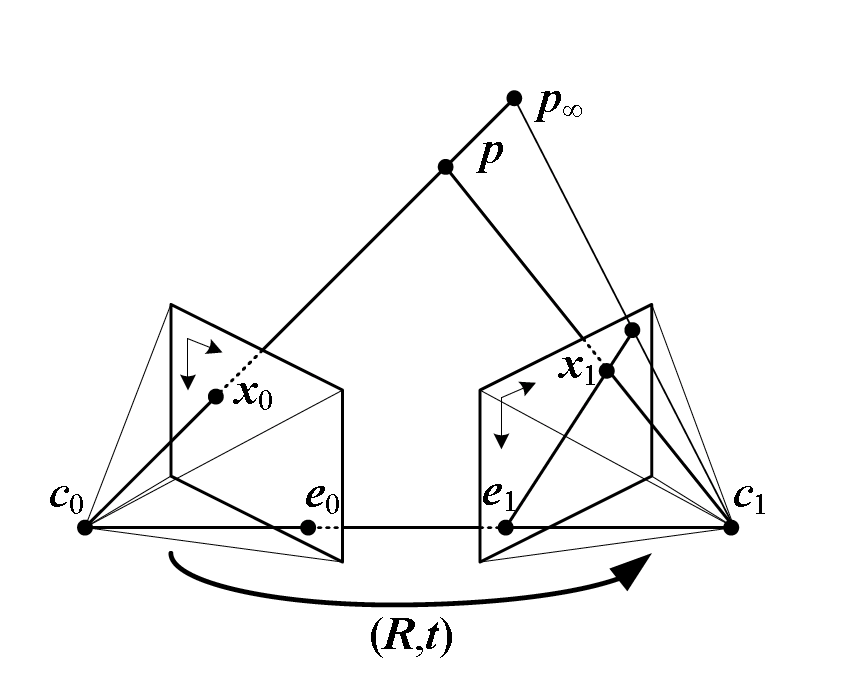
\includegraphics[width=0.40\textwidth]{./images/epipolar_1.png}
	} \qquad
	\subfloat[]{
		\label{fig:epipolar_2}
		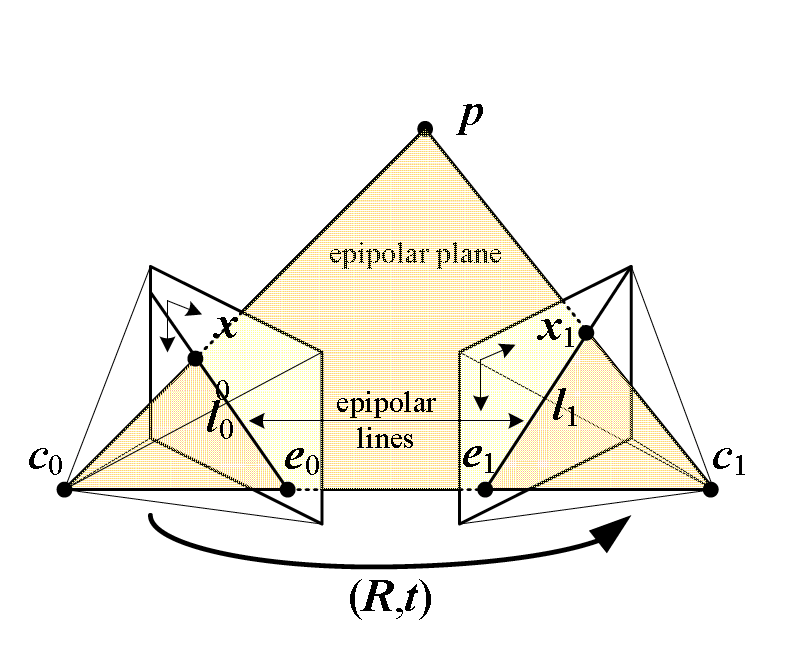
\includegraphics[width=0.40\textwidth]{./images/epipolar_2.png}
	} 
	\caption{Epipolar geometry (a) Epipolar line segment corresponding to one ray; (b) Corresponding set of epipolar lines and their epipolar plane.}
	\label{fig:epipolar}
\end{figure}

In terms of a stereo correspondence algorithm the benefit is that the search for the point corresponding to $ \rdx_{0}$ need not cover the entire image plane but can be restricted to the line $\vec{l}_{1}$. And my algorithm could also be partly proved with \textit{epipolar geometry} (seen in \cref{subsec:Rectified Stereo Images}).

\section{Least Squares Correlation}\label{sec:Least Squares Correlation}
The method of least squares is a standard approach in regression analysis to approximate the solution of over-determined systems (sets of equations which there are more equations than unknowns) by minimizing the sum of the squares of the residuals made in the results of every single equation. What's more, the least squares correlation is a very potent and flexible technique for all kinds of data matching problems. Here its detailed application process to image matching is outlined.

 Start from the most basic, linear least squares. 
\begin{definition}[Linear Least Squares]\label{thm:linear least squares}
A regression model is a linear one when the model comprises a linear combination of the parameters $\vec{\beta}=(\beta_{1}, \beta_{2}, \cdots, \beta_{n})^T$, i.e.,
\begin{align} \label{equ:model}
f(\vec{x}, \vec{\beta}) = \sum_{j=1}^{m} \beta_{j} \phi_{j}(\vec{x})
\end{align}
where the function $\phi_{j}(\vec{x}) $ is a function of input $\vec{x} = \left( x_1, x_2, \cdots, x_i\right) ^T$.

Letting $X_{ij} = \phi_{j}(x_{i})$ and putting the independent and dependent variables in matrices $X$ and $Y$ we can compute the sum of squares in the following way, note that $D$ is the set of all data: $X$ and $Y$.
\begin{align}
E(D,  \vec{\beta} ) =  \begin{Vmatrix}X\vec{\beta}- Y\end{Vmatrix}^{2}
\end{align}
Finding the minimum of it can be achieved through setting the gradient of the loss to zero and solving for $\vec{\beta}$
\begin{align}
 \frac{\partial E(D, \vec{\beta})}{\partial \vec{\beta}}  =   \frac{\partial((X\vec{\beta} - Y)^{T}(X\vec{\beta} - Y)) }{\partial \vec{\beta}}=-2X^{T}Y+2X^{T}X\vec{\beta} 
\end{align}
Finally setting the gradient of the loss to zero and solving for $\vec{\beta}$ we get:
\begin{align}
-2X^{T}Y+2X^{T}X\vec{\beta} = 0  \Rightarrow \nonumber \\
\vec{ \hat{\beta} } = (X^{T}X^{-1})^{-1}X^{T}Y
\end{align}
\end{definition}

When function $f(\vec{x}, \vec{\beta})$ represent the image mapping model, $\vec{x}$ means correspondingly the all points in the image and $\vec{\beta}$ is the parameters in the model, the process will change to an image registration process for a series of consecutive images from the video of the same scene (e.g. aerial video), since the model of image mapping according to the \cref{equ:model} is nonlinear, it is a nonlinear least square problem. This is a over-determined  problem which has more observations than the parameters.  Most algorithms involve choosing initial values for the parameters. Then, the parameters are refined iteratively i.e. the values are obtained by successive approximation. In the thesis, Gauss-Newton algorithm is used to solve this nonlinear least squares problem. 

\begin{definition}[Gauss-Newton algorithm] \label{thm:Gauss-Newton algorithm}
Given $m$ functions $\vec{r} = (r_{1}, \cdots, r_{m} )^T $(often called residuals) of n variable $\vec{\beta} = (\beta_{1}, \cdots, \beta_{n})^T $, with $m \geq n$, the Gauss-Newton algorithm iteratively finds the value of the variables that minimizes the sum of squares \cite{deuflhardLeastSquaresProblems2011}
\begin{equation}
S(\vec{\beta}) = \sum_{i=1}^m r_i^2(\vec{\beta})
\end{equation}
\end{definition}

Starting with an initial guess $\vec{\beta}^{(0)}$ for the minimum, the method proceeds by the iterations
\begin{equation}
\vec{\beta}^{(s+1)} = \vec{\beta}^{(s)} - \left(\mathbf{J_r}^{T} \mathbf{J_r} \right)^{-1} \mathbf{J_r}^{T} \vec{r}\left(\vec{\beta}^{(s)}\right)
\end{equation} 
where the entries of the Jacobian matrix it $\vec{\beta}^s$
\begin{equation}
\left(\mathbf{J_r}\right)_{ij} = \frac{\partial r_i \left(\vec{\beta}^{(s)}\right)}{\partial \beta_j}
\end{equation}

In data fitting, where the goal is to find the parameters $\vec{\beta}$ such that a given model function $y = f(\vec{x}, \vec{\beta}) $ best fits some data points$(\rdx_i,  \rdy_i)$, the function $r_i$ are the residuals:
\begin{equation}
r_i(\vec{\beta}) = y_i - f\left( \rdx_i, \vec{\beta}\right)
\end{equation}
Then, the Gauss-Newton method can be expressed in terms of the Jacobian $\mathbf{J}_f$ of the function $f$ with respect to $\vec{\beta}$ as 
\begin{equation}\label{eq:Final Gauss-Newton}
\vec{\beta}^{(s+1)} = \vec{\beta}^{(s)} + \left(\mathbf{J_f}^{T} \mathbf{J_f} \right)^{-1} \mathbf{J_f}^{T} \vec{r}\left(\vec{\beta}^{(s)}\right)
\end{equation}
Note that now the Jacobian $\mathbf{J}_f$ is for function $f$ not $r$, the sign before $\left(\mathbf{J_f}^{T} \mathbf{J_f} \right)^{-1} \mathbf{J_f}^{T} \vec{r}\left(\vec{\beta}^{(s)}\right)$ changes.




